\documentclass[9pt]{article}
\usepackage[onehalfspacing]{setspace}
\usepackage{lipsum}
\usepackage{graphicx}
\usepackage{amsmath}

\usepackage[
	backend=biber,
    style=authoryear,
    %sorting=ynt,
    bibwarn=true,
    bibencoding=utf8,
    sortlocale=de_DE,
    maxbibnames=99,
    maxcitenames=1]{biblatex}
    
\DefineBibliographyStrings{english}{
   andothers = {{et\,al\adddot}},}
   
\addbibresource{../../../bib/thesis.bib}




\begin{document}

\AtBeginEnvironment{figure}{\singlespacing}
\AtBeginEnvironment{table}{\singlespacing}

\begin{titlepage}
	\centering
	{\scshape\LARGE Ludwig-Maximilians-Universität München \par}
	{\scshape\large Department Biologie II Computational Neuroscience \par}
	\vspace{0.5cm}
	\includegraphics[width=0.7\textwidth]{../logo/GSN-Logo_ab35mmBreite_RGB.jpg}\par
	\includegraphics[width=0.4\textwidth]{../logo/siegel_black.pdf}\par
	\vspace{0.7cm}
	{\scshape\LARGE Report \par}
	\vspace{0.05cm}
	{\huge\bfseries Computational Simulation of Time Perception: Model Description and Implementation \par}
	\vspace{1.1cm}
	{\Large Katharina \textsc{Bracher} \par}
	{Student ID: 11754625 \par}
	\vspace{0.4cm}
	{\large Supervision: Dr. Kay \textsc{Thurley} \par}
\end{titlepage}


\normalsize
\tableofcontents


\section{Behavioral Effects in Magnitude Estimation}
Magnitude estimation is subject to noise that arises from external sources i.e. the statistics of the environment and internal sources i.e. neural representation of the input and the behavior.
Across sensory modalities, characteristic behavioral effects are identified (\cite{Petzschner2015}).
The most prominent observation is a regression to the mean of the stimulus range,  i.e. small stimuli are overestimated whereas large stimuli are underestimated (\textit{regression effect}). 
This effect intensifies for ranges with larger stimuli (\textit{range effect})
For larger stimuli the standard deviation of estimates increases monotonically (\textit{scalar variability}). 
Finally, the recent history of stimuli presentations influences the current stimuli estimation (\textit{sequential effect}).
All effects mentioned above are displayed in Fig. \ref{fig:behavioraleffects}. 

Modality-independence of these effects suggests the existence of a common underlying principle or processing mechanisms, that would explain e.g. a optimal strategy for unreliable judgments due to noise (in stimuli and estimates).

\begin{figure}[h]
	\centering
	\includegraphics{figures/behavioural_effects_petzschner.pdf}
	\caption{\textbf{Behavioral Effects} adapted from \cite{Petzschner2015}.}
\label{fig:behavioraleffects}
\end{figure}


\section{Model Description}
During time perception and time reproduction experiments, neural activity displays characteristic trajectories in a low-dimensional space (\cite{Meirhaeghe2021}, \cite{Wang2018}, \cite{Henke2021}). 
The neural trajectories are consistently influenced by prior beliefs. 
Flexible motor timing can be achieved by controlling the speed of neural dynamics (\cite{Sohn2019}, \cite{Wang2018}). 
Further, it has been found that neural activity in anticipation of a delayed response reaches a fixed threshold with rate inversely proportional to delay period \cite{Murakami2014}, \cite{Mita2009}).
\cite{Wang2018} proposed a potential neural mechanism for speed control and based on that \cite{Egger2020} developed a neural circuit model for sensorimotor timing.

\subsection{Circuit}
Flexible speed control can be achieved by a simple model consisting of three units, u, v, y that represent population activity. 
Two units, u and v receive symmetric input I ($W_{uI}=W_{vI}=6$) and have symmetric mutual inhibitory projections onto each other ($W_{uv}=W_{vu}=6$). 
The inputs to u and v is governed by a sigmoidal activation function $\theta(x) = \frac{1}{1+exp(-x)}$ and all three units have a time constant $\tau$ = 100. 
y is the output unit and receives excitatory input from u and inhibitory input from v ($W_{yu}=W_{yv}=1$)which results in ramp-like behavior.
Stochastic synaptic inputs are modeled as independent white noise $\eta_u, \eta_v, \eta_y$.
The dynamics of u, v, and y are defined as follows:
\begin{align} \label{circuit}
	\tau\frac{du}{dt} & = -u + \theta(W_{uI}I - W_{uv}v + \eta_u) \\
	\tau\frac{dv}{dt} & = -v + \theta(W_{vI}I - W_{vu}v + \eta_v) \\
	\tau\frac{dy}{dt} & = -y + W_{yu}u - W_{yv}v + \eta_y
	\end{align}

The speed at which the output y evolves can be controlled by the shared input to u and v (Fig. \ref{fig:circuit})c (\cite{Egger2020}) and determines the interval after which y reaches a fixed threshold $y_0$.

Depending on the input I, parameter and initial conditions, the system shows different dynamics. For low levels of I (0$<$I$<$0.5) the system has three fixed points (2 stable, 1 unstable at u=v) and y ramps up faster the higher the input I. 
For intermediate values of I (0.5$<$I$<$1) the system still shows three FP of the same sort and y ramps up with a slope that is inversely proportional to the input I (y ramps up slower the higher the input I, see schematic in Fig. \ref{fig:circuit}a, b). 
For high I (1$<$I) the system has one stable fixed point (at u=v) and y ramps down faster for higher I.
In this report, the intermediate input regime is explored. In this regime, higher a higher input I results in a smaller slope of y, such that the threshold $y_0$ is reached after a longer interval. Thus, input is controlling the speed of the dynamic. 

\begin{figure}[h]
	\centering
	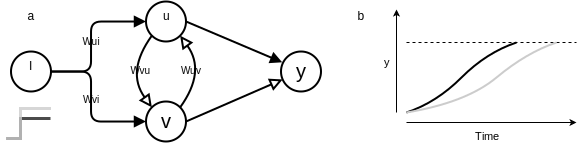
\includegraphics{figures/defCircuit.drawio.pdf}
	\caption{\textbf{Basic Circuit} \textbf{(a)} u and v share a common input I. Dynamics for example input I=0.75 in gray and I=0.65 in black plotted in (b). The input is governed by weights $W_{uI}$ and $W_{vI}$. The two units have reciprocal inhibitory connections with weights $W_{uv}$ and $W_{vu}$ that determine the inhibitory strength and project to the output unit y with an excitatory connection from u and an inhibitory connection from v. Excitatory and inhibitory connections are shown by filled and open arrows, respectively. \textbf{(b)} Dynamics of y for intermediate regime with input I=0.75 in gray and I=0.65 black. There is an inverse relation of input strength and slope. With higher input, the threshold at 0.7 (dashed line) is reached after a longer time interval. \textbf{(c)} Dynamics of u, v, y for inputs from 0.1 to 1.5. Initial conditions are set to $u_0=0.7 , v_0=0.2 , y_0=0.5$.}
\label{fig:circuit}
\end{figure}


Initial conditions of u, v and y have been optimized for in \cite{Egger2020} and are set to $u_0=0.7 , v_0=0.2 , y_0=0.5$.

\subsection{Update Mechanism and Experiment simulation}
For 
Updating I based on feedback to adjust rate in reproduction
stages: measurement, update and reset, reproduction until threshold 
update: delta y-th, weighted
parameter: memory parameter K, reset, initial conditions, 
threshold 
timeouts

\begin{align} \label{circuit}
	\tau\frac{du}{dt} & = -u + \theta(W_{uI}I - W_{uv}v + \eta_u) \\
	\tau\frac{dv}{dt} & = -v + \theta(W_{vI}I - W_{vu}v + \eta_v) \\
	\tau\frac{dy}{dt} & = -y + W_{yu}u - W_{yv}v + \eta_y
\end{align}

\section{Implementation of Model}
\subsection{Modules}
Euler Implementation to Solve Differential Equation
parallel Simulation
experiment simulation
update mechanism

\subsection{Structure of Code}
parallel simulations, experiment simulation

\section{Results and Outlook}
experiment simulation plot
behavioral plot
parameter search, extending units, neural trajectories

limitations and explorations regimes 

\end{document}